\chapter{Computing Trends}
\label{chapter:computing-trends}

\section{Modern Computing}
This chapter introduces the context of this thesis. We present the challenges and reasons that have led the traditional single threaded computing to concurrent, multi-threaded and parallelized programming, and further to a paradigms called cloud and fog computing.

The terminology around the parallelized computation is somewhat ambiguous. Throughout this chapter, we will be using the term \emph{parallel computing} as a general term referring to the opposite of \emph{single-threaded} or \emph{sequential} computing, unless explicitly stated to mean the act of \emph{parallel computing}, in which multiple calculations are carried out \emph{simultaneously}. The general term comprises many different types of computing, such as \emph{concurrent}- and \emph{distributed computing}, as well as the type of \emph{parallel computing} itself.

\subsection{The End of Free Lunch}
\label{subsection:the-end-of-free-lunch}
Until the turn of the millenium, the main drivers for the speedups in computing were the increasing CPU clock frequency and cache sizes, as well as the execution optimizations. Faster clock speeds meant that more cycles could be run in the same time, whereas the execution optimization enabled more work to be done with the same amount of cycles. Further, the increasing cache sizes kept larger parts of the computation close to the CPU cores, away from slow shared memory.~\cite{Sutter:2005:FLiO}

A notable fact about all these drivers is that, while they lead to speedups in parallel computing, they also provide direct speedups for sequential programs. Partly for this reason, until the end of 1990s, the majority of the software applications were single-threaded and sequential.~\cite{Sutter:2005:FLiO}

However, in the mid 2000s, the CPU performance gains hit the wall. Despite the fact that the transistor densities continued following the Moore's Law~\cite{Moore:1998:MooresLaw}, several physical problems limited the development of higher clock speeds. Dennard scaling, a law proposed by in 1974 stating that the power density of transistors stays constant while the transistor themselves get smaller, seems to be broken down around 2005. As the transistors got even smaller, new current leakage and chip heating problems arose and the silicon industry hit the so-called \emph{powerwall}.~\cite{Esmaeilzadeh:2011:DSE, Sutter:2005:FLiO, Ributzka:2013:Concurrency}

\begin{figure}[]
  \begin{center}
    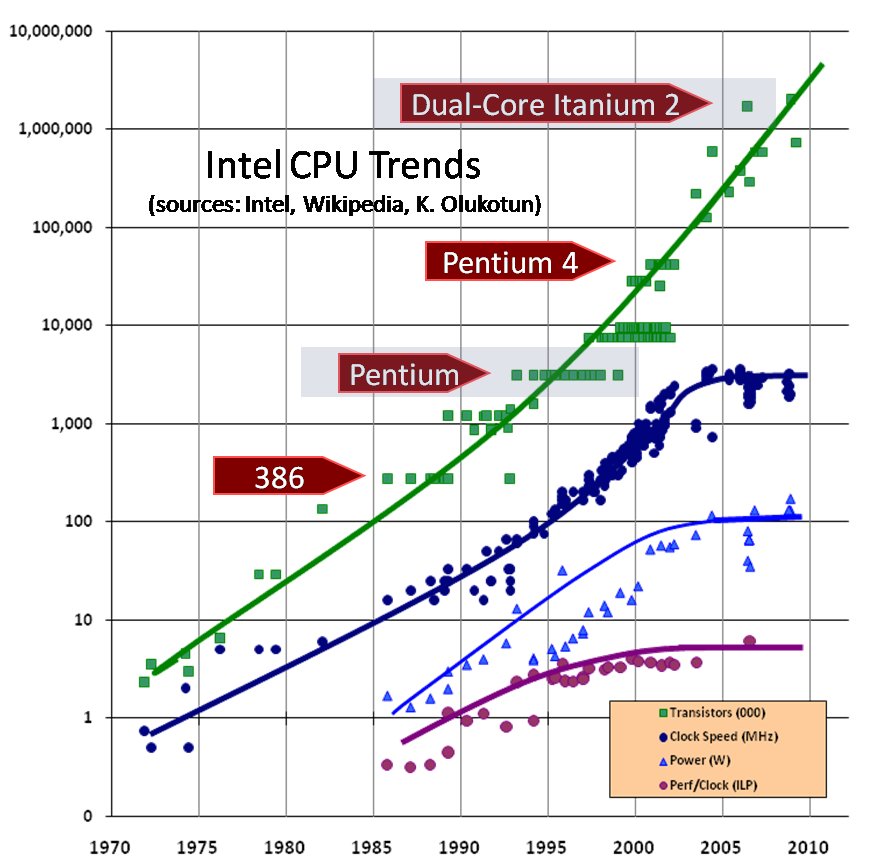
\includegraphics[width=\textwidth]{images/free-lunch-is-over.png}
    \caption{Intel CPU trends. The transistor density follows the Moore's Law, while the growth of CPU speed have stopped.~\cite{Sutter:2005:FLiO}}
    \label{fig:rne-example}
  \end{center}
\end{figure}

These chip manufacturing challenges have led into an era of \emph{dark silicon}, meaning that we cannot afford to switch all the transistors on and off at each clock cycle due to the power constraints. Before the power wall, the forefront of the silicon industry was to maximize the chip speeds. However, in the era of dark silicon, the power consumption has become perhaps the most important performance indicator, especially in the datacenter scale computing.~\cite{Sutter:2005:FLiO, Asanovic:2006:Landscape, Ributzka:2013:Concurrency, Zhang:2010:CloudComputing}

And while the silicon industry are facing various hardware development challenges, the software developers are also forced to adopt new programming paradigms to keep up with the ever increasing performance requirements.~\cite{Sutter:2005:FLiO}

\subsection{Parallel, Concurrent, and Distributed Computing}
\label{subsection:parallel-concurrent-and-distributed-computing}

The parallelization of computing has been researched for several decades. Before the sequential execution speedup gains hit the wall, it remained a minor but important field of research, mainly in high-performance computing. Parallel-, concurrent-, and distributed computing quickly became the dominant answers for mainstream computing, to continue enjoying the benefits of the exponential computing speedups.

The \emph{parallel computing type} refers to computing in which a subparts of a program are solved at the same time. \emph{Concurrent computing}, on the other hand, executes multiple computations on overlapping time periods. In \emph{distributed computing}, the overlapping or simultaneous executions are carried out on multiple computers connected to each other.

There exist many different forms of parallel computing, often divided into four high level categories: bit-level, instruction-level, task, and data parallelism. Parallelism can be implemented in both software and hardware levels.~\cite{Culler:1997:PCA}

Bit-level parallelism increases refers to increasing the processor word size, thus reducing the needed number of instructions to be executed. In instruction level parallelism, the processor executes multiple instructions at the same time. Instruction level parallelism can happen in both hardware or software level.~\cite{Culler:1997:PCA}

The data parallelism refers to the simultaneous execution of the same function, on multiple cores, across the elements of the input data. Modern graphics processing units (GPU's), often implemented as wide single instruction, multiple data (SIMD) principle, are examples of data parallelism.~\cite{Culler:1997:PCA}

In contrast to data parallelism, task parallelism refers to execution of multiple cores of (possibly) completely different functions, across the same or different input data. In a typical multi-core processor, task parallelism is achieved by executing different threads or processes, on each core.~\cite{Culler:1997:PCA}

Introducing parallelism into the computing brings various new challenges in the software development. For example, the lack of a global clock, and possible failure of components demands extensive care from the developers, on top of the already challenging software development. Different frameworks and methods have been implemented, to ease the software development of efficient parallel applications. The focus of this thesis is on task level parallelism, especially in the context of packet processing applications. We will present some of the task processing frameworks more comprehensively in subsection~\ref{sec:packet-processing}.~\cite{Asanovic:2006:Landscape}

While implementing parallel systems is challenging for software developers, there are also clear limitations in the speedup gains that these methods can achieve. Amdahl's Law states the rather obvious maxima in the speedup that the program can achieve by scaling the computation over N processors. Suppose that the parallelizable proportion of a program is P (and thus the non-parallelizable proportion being P-1), then the maximum speedup, as denoted by Amdahl's Law, is:~\cite{Amdahl:1967:VSP}

\begin{equation*}
  \frac{1}{(1-P) + \frac{P}{N}}
\end{equation*}

The implication of Amdahl's Law is that the speedup of a program is always limited by its non-parallelizable proportion, and it also brings new challenges to the utilization of the available computing resources.

\section{Virtualization}
\label{section:virtualization}
Virtualization is an act of dividing a common set of computing resources into a multiple isolated execution environments. It enables multiple operating systems to be run, in parallel, on a single processing unit, thus alleviating the efficiency problems of parallel computing.

Before the existence of multi-user operating systems and the rapid drop in hardware cost around 1980s, the virtualization was used to allow multiple users to share the same mainframe hardware. Until the end of 1990s, it remained mainly a practice of computing industry and academic research, often requiring special hardware with explicit support for virtualization. VMWare's introduction of virtualization to the x86 architecture~\cite{Walters:1999:VVP} and the personal computer industry introduced the benefits of virtualization to the wider masses.~\cite{Bugnion:2012:BVX, Barham:2003:XAV}

In the traditional, nonvirtualized system, the hardware platform resources are controlled by a single operating system. Virtualization introduces a new layer, the \emph{virtual machine monitor} (VMM), to the software stack. The VMM lies underneath the existing software components, abstracting the hardware inputs, outputs, and the behaviour for the use of multiple operating systems. The virtualized system is called a \emph{virtual machine}.~\cite{Uhlig:2005:IVT, Bugnion:2012:BVX, Barham:2003:XAV}

The benefits of the virtualization are numerous, mainly due to the software implementation of the virtual machines. It enables scalability and flexible migration of computation loads across different infrastructures, leading to improved hardware utilization, dynamic resource allocation and management, isolation, security, and automation.~\cite{Pearce:2013:VIS}

The virtual machines can be \emph{live migrated} over to another physical machine. While the nonvirtualized systems are often under utilized, the flexibility of software enables the machines often to be run on optimal usage level. Maintenance costs can be reduced by software automation and security can be increased by additional software services, such as workload isolation. These benefits have encouraged companies to seek savings, by adopting virtualization in various contexts, ranging from the desktops and datacenters to network switching.~\cite{Uhlig:2005:IVT, Pearce:2013:VIS}

To enable fully functional virtualized environments, the virtualization of different system components, such as CPU, memory, I/O, and storage, need to be considered. CPU virtualization techniques are often divided into three categories: binary translation (full virtualization), paravirtualization, and hardware-assisted virtualization.~\cite{Bugnion:2012:BVX, Pearce:2013:VIS, Horne:2007:Understanding}

Full virtualization refers to a method where the communication between the virtualized operating system (guest) and the underlying host operating system is (nearly) completely emulated, meaning that the virtual hardware is functionally identical to the underlying machine. Unmodified guest operating systems can be run similarly as on native hardware, as the virtualization layer completely decouples them from the underlying hardware. On the other hand, the complete emulation of the hardware instructions induces performance overhead to the full virtualization.~\cite{Bugnion:2012:BVX, Barham:2003:XAV, Horne:2007:Understanding}

In paravirtualization, instead of emulating the hardware environment, the guest operating systems are executed in isolated environments. It enables the communication between the guest operating system and the virtual machine monitor, and thus improving the performance and efficiency of the virutalization.~\cite{Barham:2003:XAV, Horne:2007:Understanding}

However, paravirtualization requires modifying the guest operating system kernel to enable direct communication with the virtualization layer monitor. For this reason, paravirtualization compatibility and portability is limited, and it can cause significant support and maintainability costs.~\cite{Barham:2003:XAV, Horne:2007:Understanding}

Hardware assisted virtualization introduces new hardware features to ease the virtualization. A common method is to provide a new privilage level below the ring 0, to allow the guest operating system to intercept and emulate privileged operations of the underlying hardware. Hardware assisted virtualization removes the need for binary translation and paravirtualization, thus, at least theoretically, solving many of the current virtualization problems.~\cite{Horne:2007:Understanding, Pearce:2013:VIS}


\section{Cloud Computing}
\todo[inline]{Emphasize the relationship to virtualization!}
% scale up vs. scale out
% NIST definiton of cloud computing: http://www.nist.gov/itl/cloud/upload/cloud-def-v15.pdf

Cloud computing paradigm provides a shared pool of easily configurable and flexible computing resources via convenient, on-demand network access. [3] One of the driving forces for cloud computing has been its promise of economics of scale; cloud computing centers, compared to traditional on-premise solutions, can be built using cheaper hardware, cooling, electricity, network capacity and smaller number of administrators per computer, while at the same time alleviating the problem of inefficient resource usage.~\cite{Mell:2011:ccdef}

According to the definition of The National Institute of Standards and Technology, cloud computing is composed of five essential characteristics (on-demand self-service, broad network access, resource pooling, rapid elasticity, and measured service), three service models (software as a service, platform as a service, and infrastructure as a service), and four deployment models (private cloud, public cloud, community cloud, and hybrid cloud).~\cite{Mell:2011:ccdef}

\subsection{Characteristics}
The \emph{on-demand self-service} characteristic means that the consumer of the service can provision computing resources, such as server time and network storage, automatically without requiring human interaction with each service provider. \emph{Broad network access} requires the service to be available over the network and accessible using standard mechanisms which promote use by heterogeneous platforms such as mobile phones, tablets, laptops, or personal computers. \emph{Resource pooling} refers to virtualization techniques discussed in the subsection~\ref{subsection:virtualization}. \emph{Rapid elasticity} means that the consumer is able to elastically and automatically, provision and release the seemingly untlimited resources on demand. The last characteristic, \emph{measured service}, refers to the automatic control and optimization of the resources by metering the usage of the services.~\cite{Mell:2011:ccdef}

The characteristics of cloud computing make it tempting for both customers and service providers. From the customer perspective, it provides advantages of high computing power, cheap service costs, high performance, flexible scalability and accessibility as well as high availability. It reduces the upfront infrastructure costs for companies, allowing them to focus on their core businesses instead of on infrastructure, and getting their applications running faster, with improved manageability and less maintenance. On the other hand, it provides completely new business models for the service providers.~\cite{Mell:2011:ccdef, Dikaiakos:2009:Cloud}

\subsection{Service Models}
The three service models divide the cloud services into logical levels based on the computing layers provided by the cloud service. Figure~\ref{fig:cloud-computing-service-models} presents the comparison these levels together with the on-premise solution. On-premise solution refers to model where the complete computation stack is managed by the customer.

\begin{figure}[]
  \begin{center}
    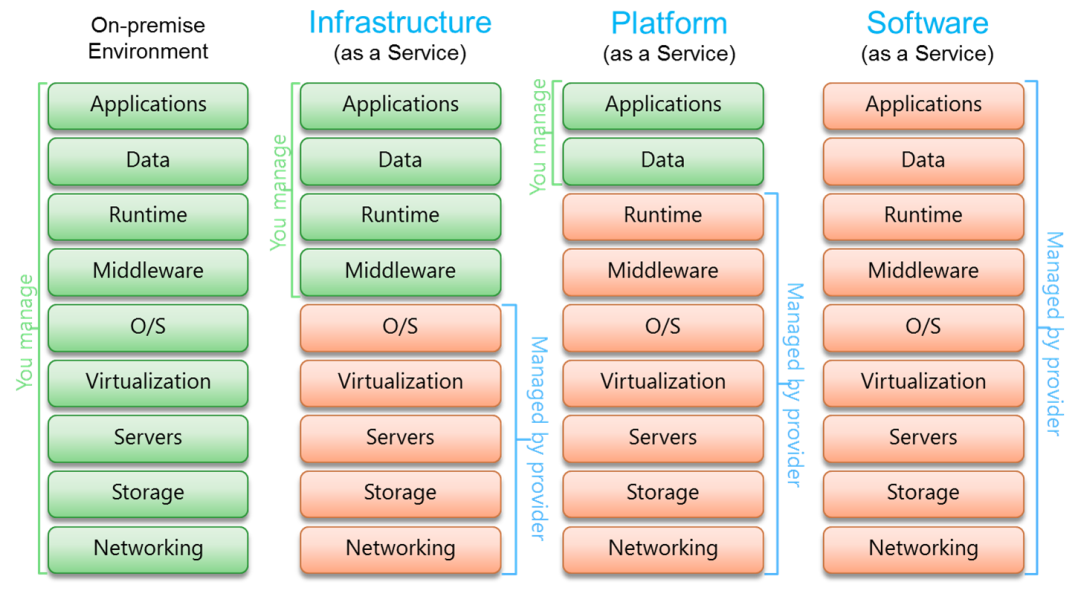
\includegraphics[width=\textwidth]{images/cloud-computing-service-models.png}
    \caption{TODO: describe the service models cite: https://www.simple-talk.com/cloud/development/a-comprehensive-introduction-to-cloud-computing/}
    \label{fig:cloud-computing-service-models}
  \end{center}
\end{figure}

The lowest of the three levels, \emph{Infrastructure as a service (IaaS)} model, provides the customer the services which abstract the details of typical hardware resources and operating systems. The computing resources are typically abstracted using a hypervisor, such as VirtualBox, KVM, Hyper-V that runs the virtual machines visible to customers as guests. Examples of IaaS providers are Amazon Web Services~\cite{Murty:2008:AWS} and Rackspace~\cite{Rackspace:2010:Inc}.~\cite{Mell:2011:ccdef}

In the next service level, \emph{Platform as a service (PaaS)} model, the service provider takes care of the platform-level middleware and runtime components. These components typically include programming-language execution environment, databases, and web servers. Google AppEngine~\cite{Sanderson:2009:GoogleAppEngine} and Windows Azure Platform~\cite{Redkar:2011:Azure} are examples of PaaS providers.~\cite{Mell:2011:ccdef}

\emph{Software as a service (SaaS)} model provides, on top of the IaaS and PaaS, the management of the application and data level. The customers access the software from cloud clients, typically web browsers via personal computers, laptops, tablets or smartphones. SaaS has become a common model for delivering wide range of different applications, such as Facebook~\cite{facebook}, Salesforce~\cite{salesforce}, and Google Gmail~\cite{Teeter:2011:Gmail}.~\cite{Mell:2011:ccdef}

\subsection{Deployment Models}
\emph{Private Cloud} infrastructure is hosted internally by a company or organization, targeting a specific set of customers. Private clouds are typically more affordable to setup and offer more flexibility, while also providing the companies full privacy on their data and applications. \emph{Public Cloud}, on the other hand, is exposed to any customer over a public network. The data, applications and other resources are stored over the service provider's data center, and thus the security has to be considered. The underlying infrastructure is often similar between these two models.~\cite{Mell:2011:ccdef}

The cloud service can also be a combination of the public and private clouds. This kind of deployment model is referred to as a \emph{hybrid cloud}. Hybrid cloud allows the utilization of the flexibility and cost of the public cloud solutions, while at the same time maintaining the security sensitive data in their own infrastructure. \emph{Community cloud} refers to cloud infrastructure that is shared between multiple organizations, typically with common security, jurisdiction, and compliance concerns in mind. Community clouds can be hosted and managed either internally or externally from the sharing organizations.~\cite{Mell:2011:ccdef}

========



% The “pay-as-you-go” Cloud Computing model is an effi-
% cient alternative to owning and managing private data centers
% (DCs) for customers facing Web applications and batch
% processing. Several factors contribute to the economy of
% scale of mega DCs: higher predictability of massive aggregation,
% which allows higher utilization without degrading
% performance; convenient location that takes advantage of
% inexpensive power; and lower OPEX achieved through the
% deployment of homogeneous compute, storage, and networking
% components.
% Cloud computing frees the enterprise and the end user
% from the specification of many details. This bliss becomes
% a problem for latency-sensitive applications, which require

To fulfill these promises, cloud computing introduces new requirements to the underlying infrastructure. Server and networking.

The development of data center technology and virtualization, together with faster telecommunication networks and proliferation of mobile devices have lad in the adoption of cloud computing.

% However, to efficiently utilize data center resources, and to provide the required performance guarantees, efficient load balancing mechanisms are needed on various locations in the data center, all the way from single server core utilization up to the efficient network routing.


% [https://www.researchgate.net/post/What_is_the_main_difference_between_Mobile_Edge_Computing_MEC_and_Fog_Computing]
% Both MEC and Fog have the goal to create a platform that provides storage, computing power, and services at the edge of the cloud rather than at the core cloud. I still confused about how to distinguish between them, rather than fog computing is a paradigm for dealing with Internet of Things (IoT).

% " Mobile cloud computing (MCC) and mobile-edge computing
% (MEC) are similar to fog computing. MCC refers to an infrastructure
% in which both the data storage and the data processing happen outside of the
% mobile devices. MEC focus on resource-rich fog servers like cloudlets running
% at the edge of mobile networks. Fog computing distinguishes itself as a more
% generalized computing paradigm especially in the context of Internet of Things."

\section{Fog Computing}
\label{section:fog-computing}
% According to [https://www.cisco.com/web/about/ac79/docs/innov/IoT_IBSG_0411FINAL.pdf], there will be 50 billion devices connected to the Internet in year 2020.
% This growth is explained by not only the growth in number of mobile devices (mobile phones and tablets, especially in developing countries)
% +!! the proliferation of IoT devices and sensors. (not included in the 50 billion)

% EMC sponsored IDC study estimates the Digital Universe to be 4.4 Zettabytes (4
% 400 000 000 TB) in 2013
% The amount of data is estimated to grow to 44 Zettabytes by 2020
% Data comes from: Video, digital images, sensor data, biological data, Internet
% sites, social media, Internet of Things, . . .
% Some examples:
% Netflix is collecting 1 PB of data per month from its video service user behaviour
% Rovio is collecting in the order of 1 TB of data per day of games logs

While the benefits of Cloud Computing provide efficient alternative to the traditional on-premise solutions, there are certain issues which have to be addressed to enable a new breed of ever demanding applications and services. Characteristics, such as mobility, geo-distribution, location awareness and low latency are intractable to achieve due to the centralized nature of cloud computing. Also, the Internet traffic volumes are growing rapidly. The proliferation of devices and sensors have led to a situation where the data are produced faster than can be transmitted or stored.~\cite{bonomi:2012:fog, vaquero:2014:FYW}

Fog computing is an extension to the traditional cloud computing architecture, where parts of the cloud computing services, mainly computation, storage, and networking, are carried out in the edge of the communication network. It is defined to provide the following characteristics on top of the existing cloud computing architectures: low latency and location awareness; wide-spread geographical distribution; mobility; very large number of nodes, predominant role of wireless access, strong presence of streaming and real time applications, heterogeneity.~\cite{bonomi:2012:fog}

High virtualization and efficient stream processing are key elements for successful fog computing.

\subsection{Data Streams}
The nature of the data in fog computing entails new types of constraints to the computing; Advanced stream processing systems are needed to process the data on-the-fly in the vicinity of the sources.~\cite{Bonomi:2012:Fog}

In the traditional von Neumann model of computing~\cite{Neumann:1993:EDVAC}, the computation is carried out by modifying the data stored in memory. However, the growing volumes of data and strict latency requirements, require not only distributing the computation, but also changes the nature of it more towards stream processing. The manipulation of the data streams passing through the system must be done on the on-the-fly.~\cite{Bonomi:2012:Fog, Thies:2002:StreamIt}

\subsection{Fog Networks}

Until recently, the typical network architectures have been implemented on proprietary or special purpose hardware. The growing networking traffic and competition in communication services have led to the development of software based solutions. Today's software based solutions are able to measure up the tight standards for stability, protocol adherence, and quality, previously achieved only with the hardware solutions.~\cite{Kim:2013:SDN}

The main enabling technologies of fog computing are the software-defined networking (SDN), and further the network functions virtualization (NFV). Software defined networking separates the data plane and the control plane functionalities of the network, making the data plane switches simple packet forwarding devices, while leaving the routing decision control logic for the control plane.~\cite{Kim:2013:SDN, Demestichas:2013:NFV}

The control plane refers to the parts of the routing architecture, that carries and consumes the control packets needed to describe the network topology and correctly route the actual data packets. The control packets originate from and are destined for a router.~\cite{Chao:2007:HPS:1202844, Yang:2004:FCE:RFC3746}

The data plane, often referred as forwarding plane, defines the part of the routing architecture, which decides destination and takes action for the data arriving to it. The decision is typically determined by a look-up table, which the incoming packet is compared to.~\cite{Chao:2007:HPS:1202844, Yang:2004:FCE:RFC3746}

SDN is often complemented with network functions virtualization. In NFV, the network devices are virtualized (using similar techniques as discussed in section~\ref{section:virtualization}) and the network functionalities of the devices are implemented in software packages.~\cite{Demestichas:2013:NFV}

Long Term Evolution (LTE)~\cite{Sesia:2009:LTE} and Evolved Packet Core (EPC) work as a natural platforms for the fog's edge data centers. Small cloud stations can be deployed to the EPCs, and the routers can be utilized as the virtualization infrastructure. This also enables the applications services to be co-located where needed.~\cite{vaquero:2014:FYW}

% The softwareisation of
% a classically hardware-driven business built around routers
% and servers where services got deployed will result in cheaper
% and more agile operations.
% The router itself becomes
% an SDN-enabled virtualisation infrastructure where
% NFV and application services are deployed close to the place
% where they are actually going to be used. But IO computing
% capabilities will still be limited (edge routers are not
% carrier grade after all).''
% ~\cite{vaquero:2014:FYW}

% The volumes of tr affic in the Internet are growing. Different sensors attached to networked systems are producing more data that can be transmitted or stored. Stream processing techniques are required to process the data streams on-the-fly. Fog computing extends the traditional Cloud computing to the edge of the communication network. Using stream processing methods in the Fog, it is possible to reduce the  pressure on transmission and storage infrastructure.

% Introduction of computational capacity to the edge of the network adds new energy consuming elements. But, the computational capacity could be used to reduce the energy consumption of a larger system. This paper studies the energy consumption of a system that uses GPUs located at the edge of the network to process video streams. The effect to the system energy consumption is compared using different communication technologies, system workloads and by deploying a Fog based filter application to limit the amount of transferred data.

% % http://www.datacenterknowledge.com/archives/2013/08/23/welcome-to-the-fog-a-new-type-of-distributed-computing/
% % Fog Computing and Its Role in the Internet of Things [http://conferences.sigcomm.org/sigcomm/2012/paper/mcc/p13.pdf]
% % https://techradar.cisco.com/technology/fog-computing#prettyPhoto

% fog computing is a paradigm that extends cloud computing to the edge of the network
% in fog computing, intelligent nodes are deployed at strategic locations of the network between the centers and the cloud
% fog computing is similar to the cloud computing, but closer to the end user, the edge, or the ground.
% scalability, reliability, faster response time, reduced cost

% fc enables capabilities that are not possible otherwise
% trains, plane, oil rig generate huge amount of data
% wireless network dont have bandwidth
% too expensive to deliver the data
% sending packet from end user to cloud might be too slow
% manufacturing: decision need to be made in fractions of seconds
% bring processing to the data, not vice versa

% improved reliability:
% network connection to the cloud goes down -> decisions can still be made
% fog computing does not contradict cloud computing, nor replace it, it complements it with much needed compute, storage and networking capabilities, at stratetig loc between sensors and data
% real-time analytics, machine learning algorithms
% analytics and ml algorithms are essential ingredients in many fog computing applications
% data into actionable insights and BI

% huge business opportunity

% % Finding your Way in the Fog: Towards a Comprehensive Definition of Fog Computing [http://delivery.acm.org/10.1145/2680000/2677052/p27-vaquero.pdf?ip=130.233.87.116&id=2677052&acc=ACTIVE%20SERVICE&key=74A0E95D84AAE420%2E1D2200B0A299939C%2E4D4702B0C3E38B35%2E4D4702B0C3E38B35&CFID=562969494&CFTOKEN=64137578&__acm__=1448197233_c568466fa204a88d9106d97b20594a8d]
% A definition for fog
% challenges: privacy, volatility, bandwidth, mobility, billions of devices

\section{Packet Processing}
\label{sec:packet-processing}
Packet processing refers to the methods applied to transport the data packets through the various network elements of the communication network. The network routers, switchs, and other elements such as computers and smartphones have their own packet processing subsystems to manage the packet traversal between the network elements.

The packet processing is divided into multiple abstraction layers, which define and stadardize the communication functions between the physical transfer level and the application level of a system. Widely adopted Open Systems Interconnection model (OSI) partitions the communication system into seven abstraction layers.



\subsection{Fast path Architecture}
Fully packet based architectures are becoming more common in every part of the data communication networks. This, together with the introduction of increasing Ethernet speeds introduces strict requirements to the electronic network elements. While the control- and management planes will require non-trivial solutions, the main bottleneck, to keep up with the scalability of optical transmission technology, seems to be the data plane processing.~\cite{Hauger:2009:PP}

The comparison of the speeds of Ethernet based transport networks and the processor speeds gives a perspective of the data path processing requirements. A typical Ethernet link with 100Gbps speed and minimum frame size of 64 bytes, leaves the packet processing system 6.7ns to process each packet. Completely software based solutions are insufficient to answer these requirements.~\cite{Hauger:2009:PP}

Fast path architecture refers to an path through a computer program, which incorporates smaller number of instructions or other optimization methods, compared to the 'normal path'. In packet processing systems, only minority of the data require complex processing. Thus, the data plane processing is often split into two layers: fast path and slow path.~\cite{cavium:2010:fundamentals, 6wind:2016:FP}

The typical slow path of the data plane is run on top of an operating system stack. The fast path layer processes packet outside the operating system environment, often with hardware acceleration, thus avoiding the overheads occuring from the thick software stack. This leaves only a small number of packets, that require special processing, to be forwarded to the slow path able to do more complex processing. Typical examples of packets requiring slow path handling are IP options and ARP packets. In MPSoC packet processing systems, such as Cavium OCTEON II CN6880, the processing cores can often be dynamically configured to run fast path or slow path.~\cite{cavium:2010:fundamentals, 6wind:2016:FP}

\subsection{Data Plane Development Kit}
\todo[inline]{clean API with a set of coherent libraries and drivers}

\todo[inline]{generic support for many CPUs/NICs}
\todo[inline]{easy to use and understand}
\todo[inline]{documentation}

\todo[inline]{DPDK subscribers/commits}

\todo[inline]{Many of today's dataplane architectures use run to completion model. No cycles can be wasted for scheduling. Applications poll for received packets. Power management?}

\todo[inline]{poll mode drivers}

\todo[inline]{DPDK almost ISA neutral, but has to be done properly}

\todo[inline]{DPDK: Hugepages -> less TLB cache misses}

\todo[inline]{Legacy dataplane? Legacy IPsec?}

\todo[inline]{Protocols, addresses, ports, packet dropping, flow reordering}
\todo[inline]{Reference implementations: Intel DPDK, ODP}
\subsection{OpenDataPlane}
\subsection{Open Event-Machine}
% TODO:
% - vs. löytyykö vielä jotain muita task processing malleja jotka samankaltaisia kuin OpenEM?
% - onko missään näistä tukea hajautetulle laskennalle?

% The OpenEM framework provides a programming model for scalable and dynamically load balanced applications. The key components of the OpenEM programming model are events, execution objects, queues and the scheduler. OpenEM operates with so-called run-to-completion principle. The run-to- completion principle means that once an event starts executing it will not be interrupted. New events cannot be scheduled until a core has completed its current task even if the events in execution had lower priorities than the events forced to wait. This implies limitations within which well performing applications must be designed. The program has to be divided to small events, so that the scheduler may efficiently distribute the computation and adhere to scheduling rules and priorities. Another limitation implied by the run-to-completion principle is that application needs to be implemented lock- free for good performance. [26]

% The OpenEM framework structure and functionality are loosely defined by the source code distribution available at [26]. Apart from the source dis- tribution, there exists no public declaration of the structure and functionality of the framework. This lack of detail is explained by the OpenEM design principles, which are stated in the OpenEM source files at [26]. A selection of the design principles is presented here. The following list is not in any particular order.

% - OpenEM has been designed to be easy to implement on different mul- ticore SoCs.
% - Easy integration with modern hardware accelerators is stated to have been a major driver in the OpenEM concept design.
% - All of the calls in the OpenEM API are multicore safe meaning no data structure gets broken if multiple cores make calls simultaneously. However the application designer needs to take the parallelism into con- sideration with regards to the application data structures and execution order.
% - The API attempts to guide the application designer towards portable architecture.
% - The API is not defined for portability through recompilation.
% - OpenEM does not implement a full software platform or a middleware solution. OpenEM implements a driver-level layer of such a solution but can be used by the application directly for best performance.

% Another factor explaining the loose definitions is how NSN views the status of its own public OpenEM implementation targeted for Intel DPDK. The disclaimer in the NSN source distribution at [26] states: ``The implementation of OpenEM for Intel CPUs in this package should NOT be considered a Reference OpenEM implementation'', but rather an ``Example of an all-SW implementation of OpenEM for Intel CPU'' This helps put the differences between the OpenEM API specification and the TI OpenEM implementation introduced in 3.2 in context.

Queues, Execution Objects, Scheduler

\todo[inline]{vs. Intel DPDK, ODP??}
\todo[inline]{Mapping between fast path hardware and dataplane application}
\todo[inline]{Event driven parallel programming model}
\todo[inline]{Currently no support for distributed computation}

% \section{Mobile-edge Computing}
% Use cases:
% Device location tracking
% Agumented Reality Content Delivery
% Video Analytics
% Radio Access Network (RAN) -aware Content Optimization
% Distributed Content and DNS caching
% Application-aware Performance Optimization

% Edge: at the base station or at the aggregation point? ETSI specification mentions both!
%   - at base station, the mec would provide minimal latency
%   - at aggregation point, the solution can be more cost effective

% World's first content delivery network (CDN): http://www.saguna.net/news-events/press-releases/saguna-and-akamai-showcase-the-world-s-first-content-delivery-network-operating-from-the-mobile-base-station/?utm_source=Blog?utm_medium=website?utm_campaign=Q2-2015

% PERFORMANCE PARAMETERS!

% !!Service-oriented Architecture (SOA)

% Load balancing problems and congestion on all the levels

% In cloud environment, the computing nodes are heterogeneous
% -> Load balancing is very important, but complex

% CIA model!
% CAP model?
% SNMP protocol?

% ``Move the computation code to the data, not the other way''

% CPU bound vs. IO bound: Florence at al. Energy Aware Load Balancing for Computational Cloud

% ``Cloud computing is the key mantra of today’s technology
% era. It caters anything as a service. It promotes resource
% sharing through internet. Eventually in cloud computing load
% balancing is a major concern used to allocate the tasks across
% several computers. Major concerns of load balancing are:
% optimal resource utilization, maximize processor throughput,
% minimize task response time, and avoid overloading''

% ``To achieve maximum throughput, in turn to improve the
% overall system performance [3], tasks can be migrated from
% overloaded nodes to lightly loaded nodes. In a cloud
% environment, to enhance the system performance workload is
% divided effectively across the participating nodes[5].There are
% two types of load balancing algorithms [9] existing such as:
% - Static – It is non-preemptive. The master distributes the
% workload between the slaves according to their
% performance.Once a host is allocated for a process, it
% cannot be pre-empted at run time. Here workload
% allocation is static.
% - Dynamic –Work load is distributed at run time
% dynamically. Processes are migrated dynamically from
% over loaded nodes to under loaded nodes in order to
% keep all the nodes busy with balanced load.''

% % [1] M. Kocaoglu, D. Malak, O. Akan, “Fundamentals of Green Communications and Computing: Modeling and Simulation,” Computer, Vol. 45, pp. 40-46, July 2012.
% % [7] K. Abbas, F. Zarafshan, Adznan, B. Jantan, “A New Fuzzy Approach  for Dynamic Load Balancing Algorithm,” International Journal of Computer Science and Information Security, Vol. 6, pp. 1-5, 2009.
% % [11] George Cybenko, “Dynamic Load Balancing for Distributed Memory Multiprocessors,” Journal of Parallel and Distributed Computing, Vol. 7, pp. 279-301, 1989.
% % [12] A.H.Harp, “Programming for Parallelism”, IEEE Computer, Vol. 20, pp. 41 – 47, 1987.
% %https://portal.etsi.org/Portals/0/TBpages/MEC/Docs/Mobile-edge_Computing_-_Introductory_Technical_White_Paper_V1%2018-09-14.pdf

% ``Load balancing is a core networking solution responsible for distributing incoming traffic among servers hosting the same application content. By balancing application requests across multiple servers, a load balancer prevents any application server from becoming a single point of failure, thus improving overall application availability and responsiveness. For example, when one application server becomes unavailable, the load balancer simply directs all new application requests to other available servers in the pool.

% Load balancers also improve server utilization and maximize availability. Load balancing is the most straightforward method of scaling out an application server infrastructure. As application demand increases, new servers can be easily added to the resource pool, and the load balancer will immediately begin sending traffic to the new server.

% Early generation server load balancers are tried and true solutions for improving the availability and scalability of an organization’s application infrastructure. Nonetheless, enterprises that persist in using such products run the risk of exposing themselves and their customers to increasingly poor application performance and a seemingly endless stream of application layer security threats.''
% % https://www.citrix.com/glossary/load-balancing.html

% Proactive vs. reactive

% % https://www.usenix.org/legacy/event/hotice11/tech/full_papers/Wang_Richard.pdf
% % [5] S.Lee,R.Panigrahy,V.Prabhakaran,V.Ramasubramanian,K.Talwar,L.Uyeda, U.Wieder,Validatingheuristicsforvirtualmachinesconsolidation,Technical Report,2011.
% % [6] M. Sindelar, R.K. Sitaraman, P. Shenoy, Sharing-aware algorithms for virtual machine colocation, in: Proc. of the 23rd ACM Symposium on Parallelism in AlgorithmsandArchitectures,SPAA’11,2011.
% % [7] C. Isci, J.E. Hanson, I. Whalley, M. Steinder, J.O. Kephart, Runtime demand estimation for effective dynamic resource management, in: Proc. of the IEEE NetworkOperationsandManagementSymposium,NOMS,2010.
% % https://www.cct.lsu.edu/~xuelin/openflow/sigcomm09-demo-loadbalancer.pdf

% % !! http://www.cs.yale.edu/homes/jf/nox.pdf

% % laja Load-balancing viitteita:
% % Zhang et al. Web server load balancing: A queueing analysis

% Centralized. vs. distributed load balancing
%   - centralized creates overhead, but provides better overview
%   - in centralized design, the network is more fault toleranec
% static vs. dynamic load balancing
% cloud vs. grid. vs. cluster

% eucalyptus greedy first-fit with round-robin vm mapping

% % [15] Lee, R. & Jeng, B. (2011). Load-balancing tactics in cloud . In proc. International Conference on Cyber- Enabled Distributed Computing and Knowledge Discovery (CyberC), IEEE, (pp. 447-454).
% % [16] Wang, S. C., Yan, K. Q., Liao, W. P. & Wang, S. S. (2010). Towards a load balancing in a three- level cloud computing network . Proceedings of 3 rd International Conference on Computer Science and Information Technology (ICCSIT), IEEE, July, 1, 108-113

% % A Comparative Study of Load Balancing Algorithms in Cloud Computing Environment
% % http://arxiv.org/pdf/1403.6918.pdf

% % OpenStack: Toward an Open-Source Solution for Cloud Computing [http://citeseerx.ist.psu.edu/viewdoc/download?doi=10.1.1.245.229&rep=rep1&type=pdf]


% Unified computing system: https://kemptechnologies.com/server-load-balancing-appliances/loadmaster-for-ucs/overview/

% ``Cloud computing promises to increase the velocity with which applications are deployed, enhance
% modernization, and lower expenses, all at the same time increasing business agility. Cloud Computing is a
% concept that has many computers interconnected through a real time network like internet. Cloud computing
% mainly refers to distributed computing. Cloud computing enables well-situated, on-demand, dynamic and
% reliable utilization of distributed computing assets. The cloud is altering our life by providing users with new
% kinds of services. Users acquire service from a cloud without paying attention to the details. Cloud computing is
% a on demand service in which shared resources work together to perform a task to get the results in minimum
% possible time by distribution of any dataset among all the connected processing units. Cloud computing is also
% referred to refer the network based services which give an illusion of providing a real server hardware but in real
% it is simulated by the software's running on one or more real machines. Such virtual servers do not exist
% physically so they can be scaled up and down at any point of time [1]. Cloud computing is high utility software
% having the ability to change the IT software industry and making the software even more attractive [2]. Hence, It
% helps to accommodate changes in demand and helps any organization in avoiding the capital costs of software
% and hardware [3] [4]''
% % <-Haryani, Jagli: Dynamic Method for Load Balancing in Cloud Computing

% % https://f5.com/resources/white-papers/cloud-balancing-the-evolution-of-global-server-load-balancing

% % Load Balancing in the Cloud Computing Using Virtual Machine Migration: A Review [http://www.ijaiem.org/volume3issue5/IJAIEM-2014-05-31-131.pdf]

% % Load Balancing Cloud Computing: State of Art [http://ieeexplore.ieee.org/stamp/stamp.jsp?arnumber=6249253]

% % Join-Idle-Queue: A novel load balancing algorithm for dynamically scalable web services [http://dl.acm.org/citation.cfm?id=2039718]


% In~\ref{churhc et al. On Delivering Embarrassingly Distributed Cloud Services} Church et al. highlight the advantages of small scale data centers over a mega centers.

% % An architecture for Load Balancing Techniques for Fog Computing Environment  [http://csjournals.com/IJCSC/PDF6-2/43.%20Manisha.pdf]

% % Cisco: [http://www.cisco.com/c/en/us/td/docs/solutions/Enterprise/Data_Center/VMDC/ASA_Cluster/ASA_Cluster/ASA_Cluster.html]

% `` Hierarchical Network Layers

% The data center within the VMDC reference architecture is based on the classic multi-layer hierarchical network model. Hierarchical model benefits include scalability, resilience, performance, maintainability, and manageability and its design represents a structured approach to building the infrastructure, allowing for relatively easy expansion in modular increments. Redundant nodes and links at each level insure no single point of failure, while link aggregation can be engineered for optimal bandwidth and performance through the aggregation and core layers. In general, this hierarchical model uses three layers:

% •Core Layer—Characterized by a high degree of redundancy and bandwidth capacity and thus optimized for availability and performance.

% •Aggregation Layer—Characterized by a high degree of high-bandwidth port density capacity and thus optimized for traffic distribution and link fan-out capabilities to access layer switches. Functionally, the nodes in the aggregation layer typically serve as the Layer 2/Layer 3 boundary.

% •Access Layer—Serves to connect hosts to the infrastructure, providing network access, typically at Layer 2 (L2) (i.e., LANs or VLANs).''

% http://web.stanford.edu/class/ee380/Abstracts/091118-DataCenterSwitch.pdf

% % A Scalable Commodity Data Center Network Architecture,
% % Data Center Switch Architecture in the Age of Merchant Silicon
% % PortLand: A Scalable Fault Tolerant Layer 2 Data Center Network Fabric

% % http://ccr.sigcomm.org/online/files/p63-alfares.pdf


% The goal of load balancing system is to provide optimal resource, e.g. central processing units, memory, or storage, utilization and desired performance metrics, usually maximal throughput, minimizing response time, and avoiding congestion and overloading parts of the system.

% Traditional web server load balancing algorithms are not sufficient for the large scale and distinct structure of so-called service-oriented data centers.

% One on the main requirements for cloud, or fog, computing is efficient load-balancing.
% Telecommunication industry is facing difficult challenges to keep up with more demanding needs of end users and businesses.
% \begin{itemize}
% \item end users need:
%   \item personalization
%   \item performance
%   \item ux
% \item businesses need:
%   \item information from consumers
%   \item easier, secure access to devices
%   \item more flexible provisioning of new services
% \end{itemize}

% Mobile traffic has been growing, and no end to that is in sight. number of sensor expected to grow exponentially. cellular network is becoming uniquitous.
% \begin{itemize}
% \item IOT, huge amount of (wireless) sensors
% \item MACHINE TO MACHINE!
% \item smart phones
% \item streaming video
% \item messaging
% \item P2P
% \end{itemize}

% The IT and Telecommunication Networking evolutions are coming closer to each other.
% -> new possibilities
% -> computation is moving to the network edge, closer to the end user and sensors.

% ``Mobile-edge Computing can be seen as a cloud server running at the edge of a mobile network and performing specific tasks that could not be achieved with traditional network infrastructure. Machine-to-Machine gateway and control functions are one example, but there are many others.''

%%% Local Variables:
%%% mode: latex
%%% TeX-master: "thesis-hartikainen"
%%% End:
